\subsection{Iteration \#2}
I iteration 2 er formålet at færdiggøre funktionalitet på websitet så det muliggøres at oprette nye waypoints til dronen og at muliggøre autonome flyvning. Bruger skal kunne oprette flyveopsætninger og gøre dem tilgængelig for dronen, hvilket kræver yderlige kommunikations opsætning hos mellem drone. Ydermere skal dronen kunne finde egen GPS position, flyvehøjde og orientering. Ud fra viden om egen position, flyvehøjde og orientering skal dronen flyve til de lokationer som er fastsat i flyveopsætningen. 
Hvordan systemet er tiltænkt at bruges beskrives i user story nedenfor:

\subsubsection*{User story}
Bruger logger på webapplikationen med sit brugernavn og password. Når der er logget korrekt ind vises bruger sin eller sine droner på en liste. Ved at trykke på en drone vises bruger information om den pågældende drone. Informationen beståer af waypoints, om der skal tages billeder ved de forskellige waypoints samt indstilling af flyvehøjde. Brugeren klikker på en drone fra listen og derefter klikker på kortet for at oprette waypoints, i det waypoints bliver oprettet bliver et nyt event også oprettet. Brugeren giver eventet et navn og en kommentar og trykker på knappen "publish to drone".
Når en drone er tændt og færdig initialiseret fortæller den server webserveren om sin nuværende position og kontrollerer om en ny flyveopsætning er tilgængelig. Er der en ny flyveopsætning tilgængelig hentes den og dronen påbegynder flyvning.

%kommentar
\begin{figure}[H]
	\centering
	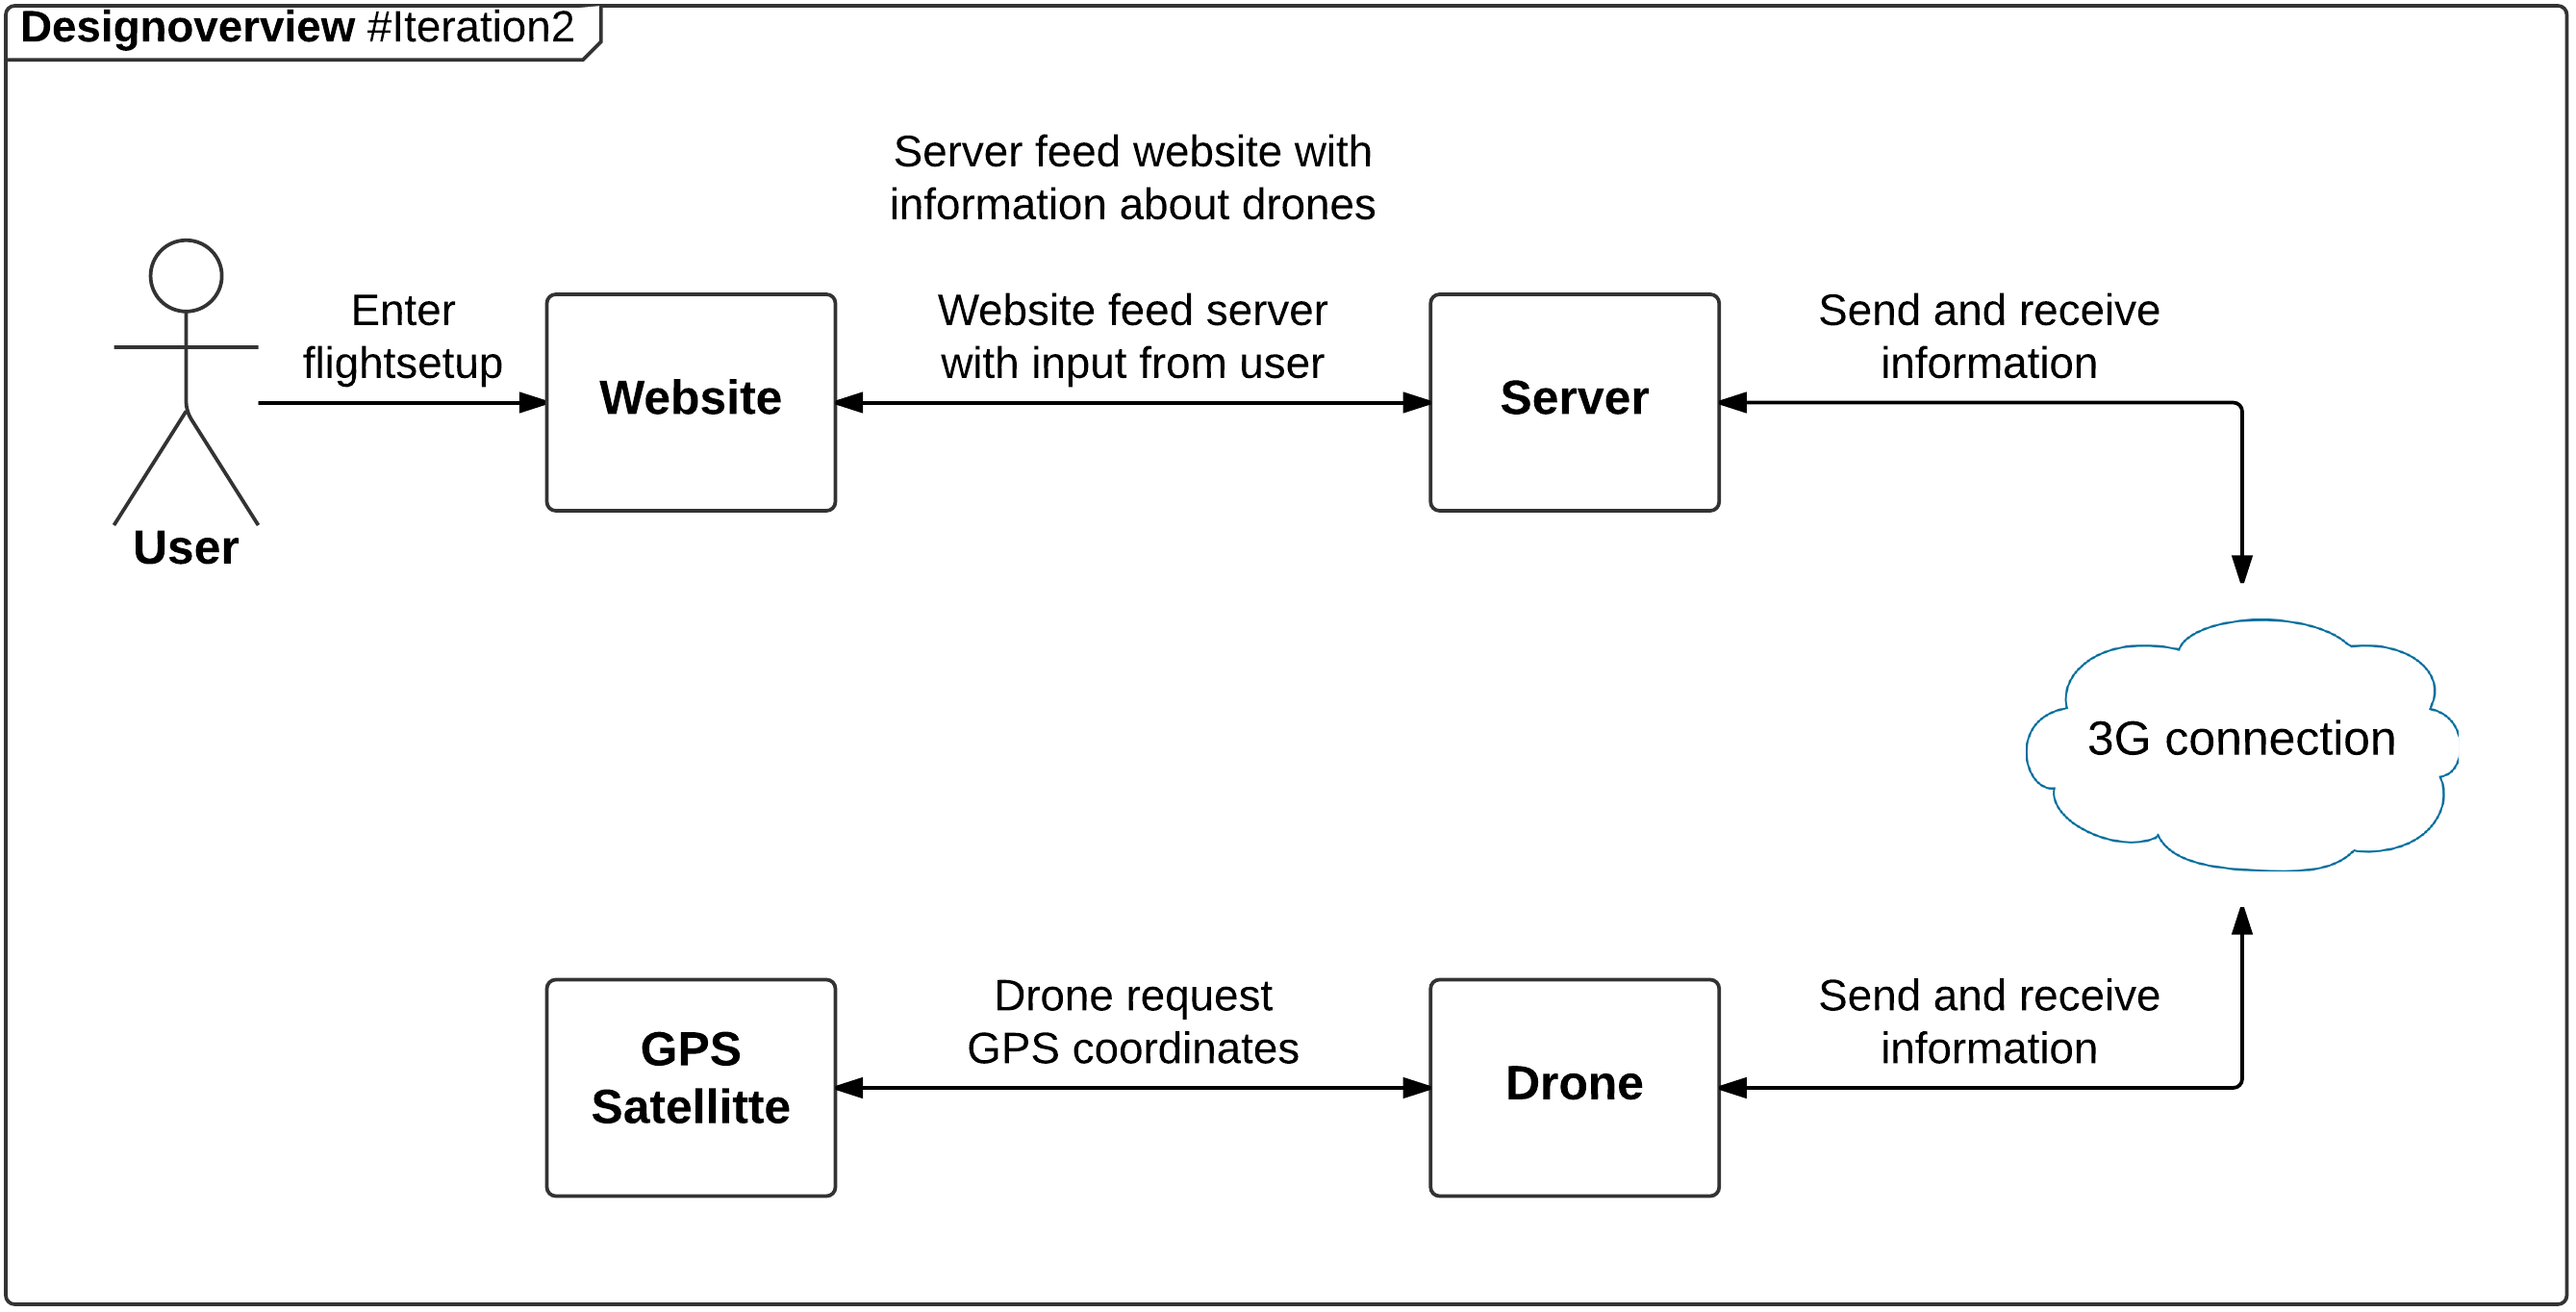
\includegraphics[width=1\textwidth]{Billeder/design_overview/design_overview_iteration2.png}
	\vspace{-.5cm}
	\caption{Designoverview \#iteration 2}
	\label{fig:design_overview_UC1}
\end{figure}



\newpage

\subsubsection*{Sekvens diagram}

Til iteration 2 er systemsekvensen beskrevet med 3 mindre sekvensdiagrammer i stedet for 1 stort. 
Denne fremstilling gør det muligt at repræsentere systemets funktionalitet på mere overskuelig vis, hvilket burde gøre indirekte øger forståelsen af diagrammerne. Hvert af de 3 sekvensdiagrammet bruges til at fortælle hvordan en delmængde af systemet fungerer.

Af figur \ref{fig:Sekvens_diagram_iteration2_1} fremgår det hvordan bruger opretter en ny flyveopsætning. Det vises desuden hvilke interaktioner der foretages mellem bruger og website, samt hvordan server løbende indgår og benyttes i sekvensen. 

%kommentar
\begin{figure}[H]
	\centering
	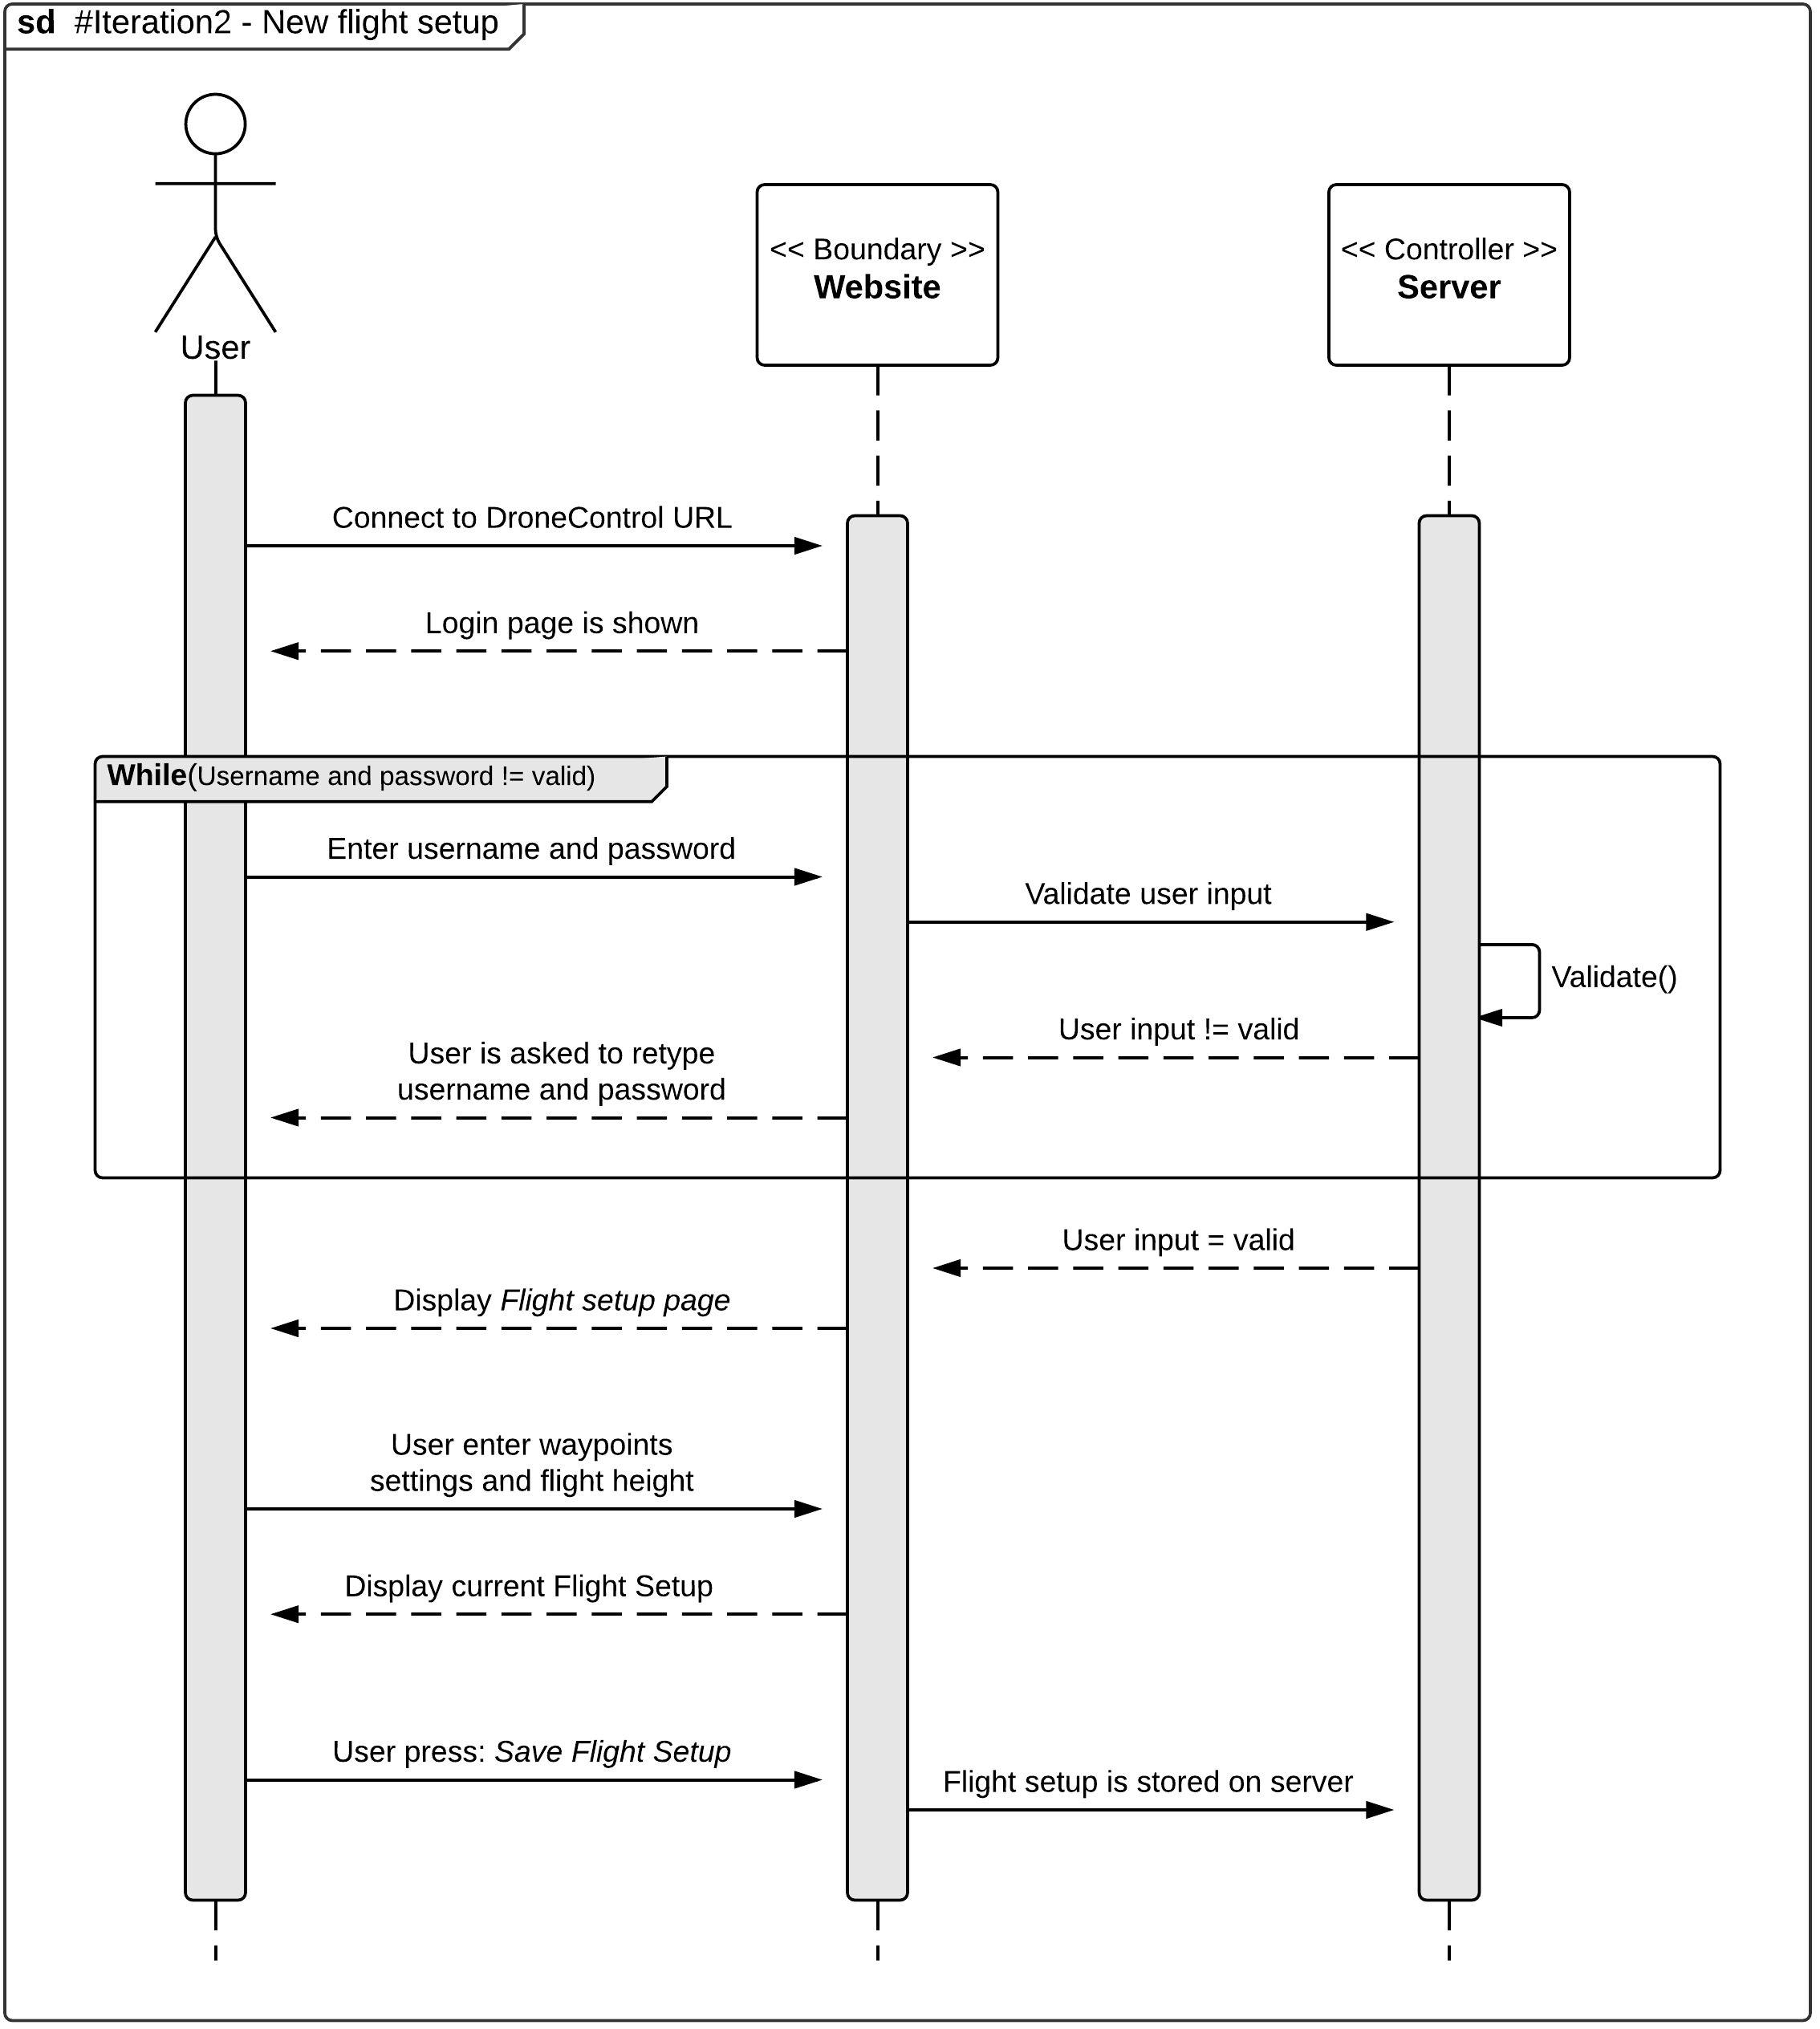
\includegraphics[width=1\textwidth]{Billeder/sekvens/sekvens_iteration2_1}
	\caption{Sekvensdiagram \#iteration 2}
	\label{fig:Sekvens_diagram_iteration2_1}
\end{figure}


\newpage

På figur \ref{fig:Sekvens_diagram_iteration2_2} fremgår det hvordan dronens main controller via 3G-shieldet kommunikerer med serveren for at kontrollere om der er en ny flyveopsætning tilgængelig. Det vises også hvilke beskeder der flyder frem og tilbage mellem main controller og server. Desuden vises det at dronen først henter ny flyveomsætning, når serveren har bekræftet, at der er en flyveopsætning tilgængelig.   

%kommentar
\begin{figure}[H]
	\centering
	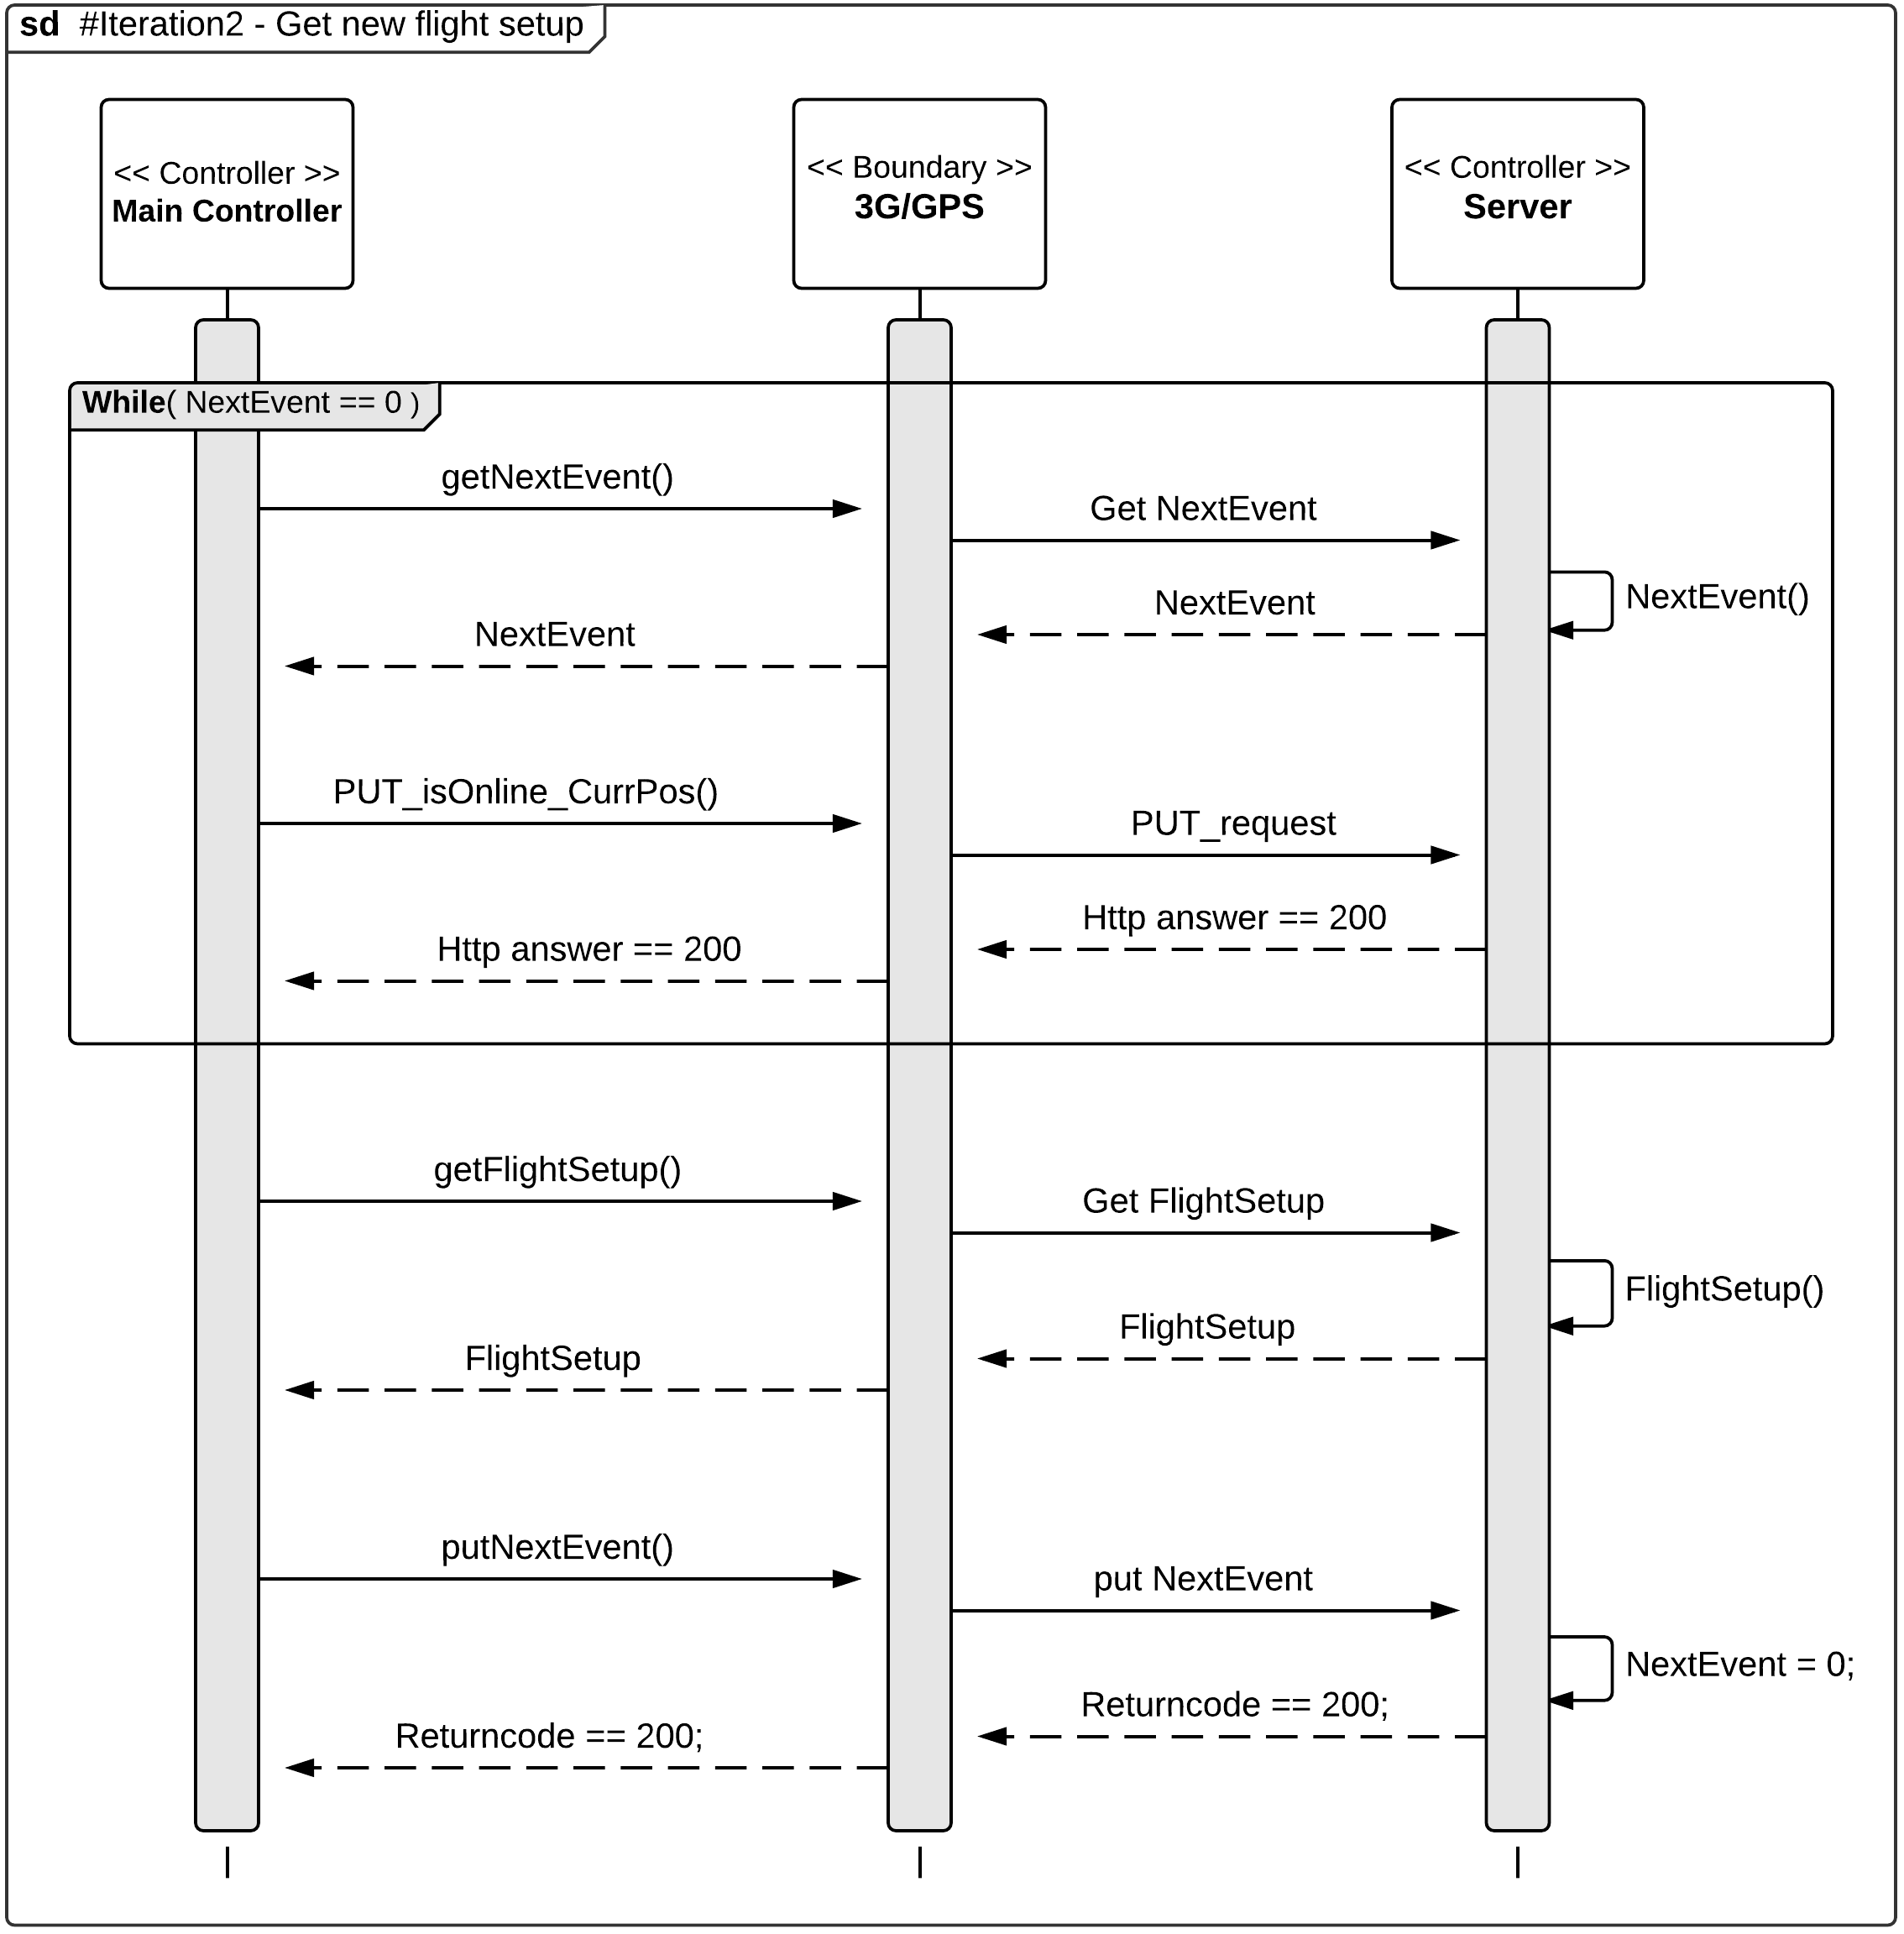
\includegraphics[width=1\textwidth]{Billeder/sekvens/sekvens_iteration2_2}
	\caption{Sekvensdiagram \#iteration 2}
	\label{fig:Sekvens_diagram_iteration2_2}
\end{figure}

\newpage

Af figur \ref{fig:Sekvens_diagram_iteration2_3} fremgår det hvordan dronen opererer når den flyver autonomt mod en givet GPS position. Main controlleren indsamler kompas data fra flight control boardet, latitude og longitude fra 3G/GPS modulet og flyvehøjde fra ultralyds sensoren. Den indhentede data processeres og bruges til at korrigerer de nuværende flyveindstillinger.
Som det fremgår af while loopet fortsætter flyvningen indtil dronen er 15 meter fra den GPS bruger valgte i flyveopsætningen. 


%kommentar
\begin{figure}[H]
	\centering
	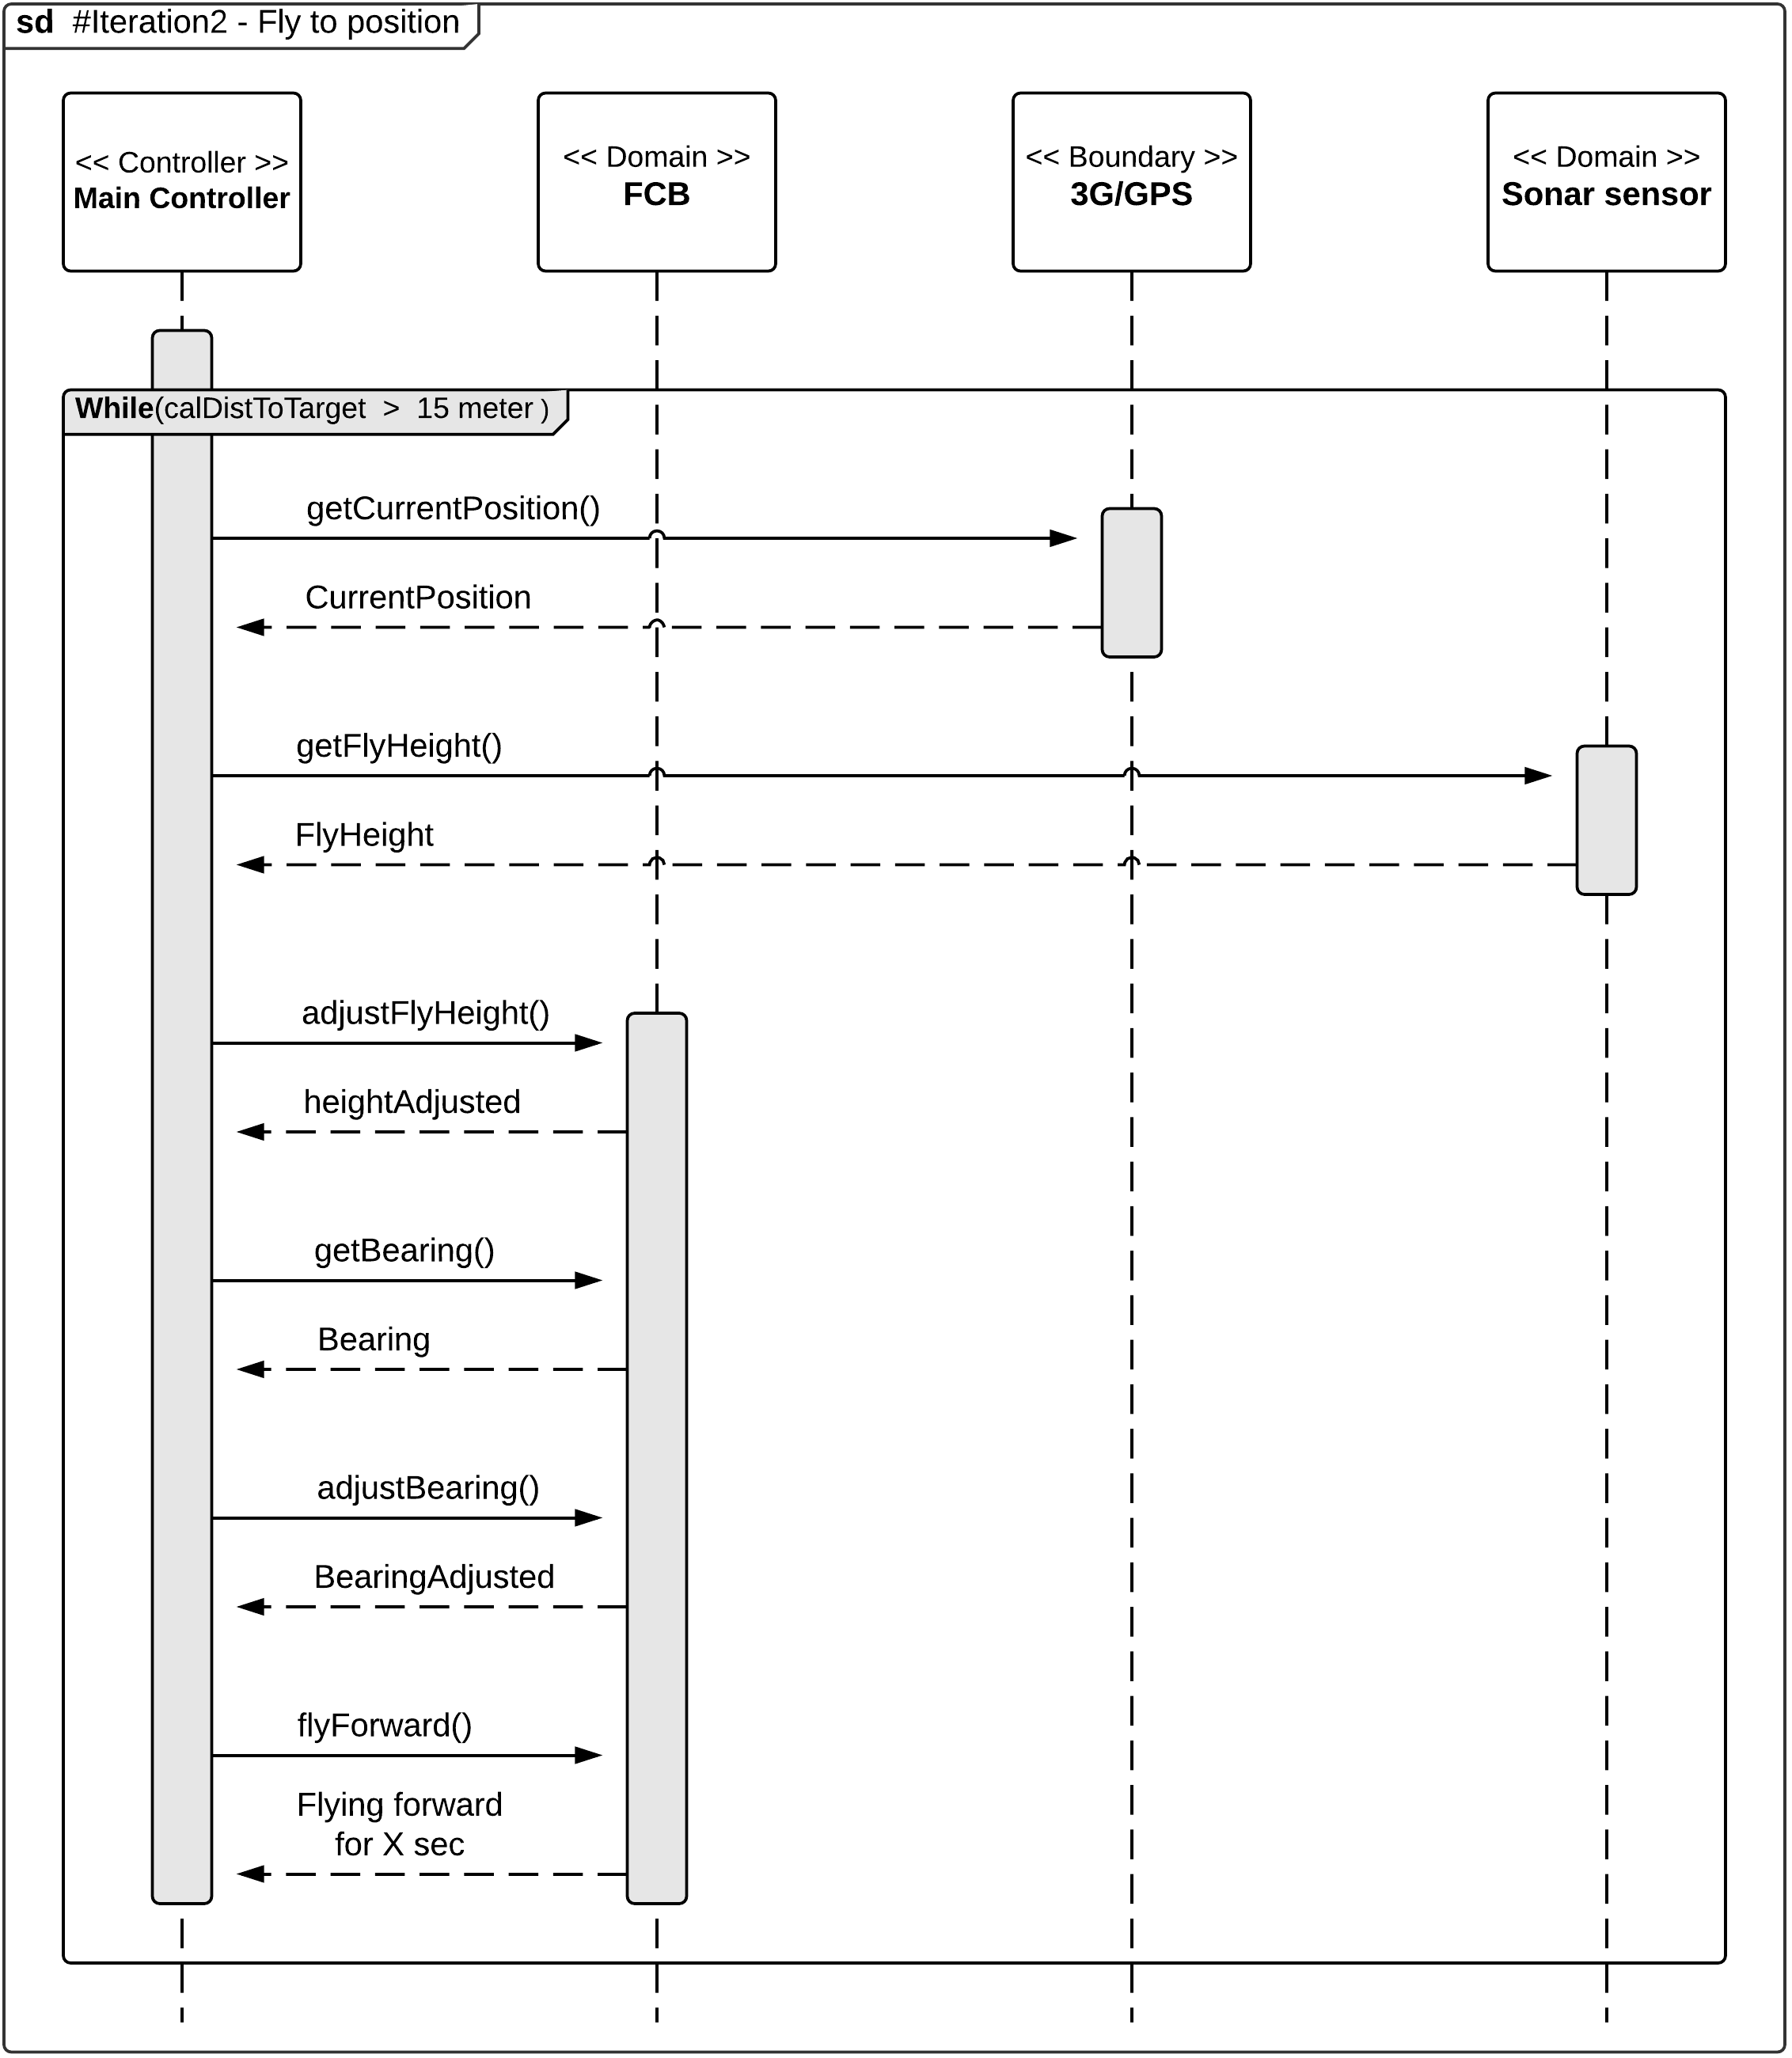
\includegraphics[width=1\textwidth]{Billeder/sekvens/sekvens_iteration2_3}
	\caption{Sekvensdiagram \#iteration 2}
	\label{fig:Sekvens_diagram_iteration2_3}
\end{figure}

\newpage
\subsubsection*{Klasse diagram - website}
\vspace{-0.1cm}
På figur \ref{fig:classDiagram_home} ses klasse diagrammet tilhørende iteration to for websitet. Funktionaliteten er blevet udvidet med overblik over droner i systemet og deres status. Mulighed for at oprette events til den ønskede drone. 
\begin{figure}[H]
	\centering
	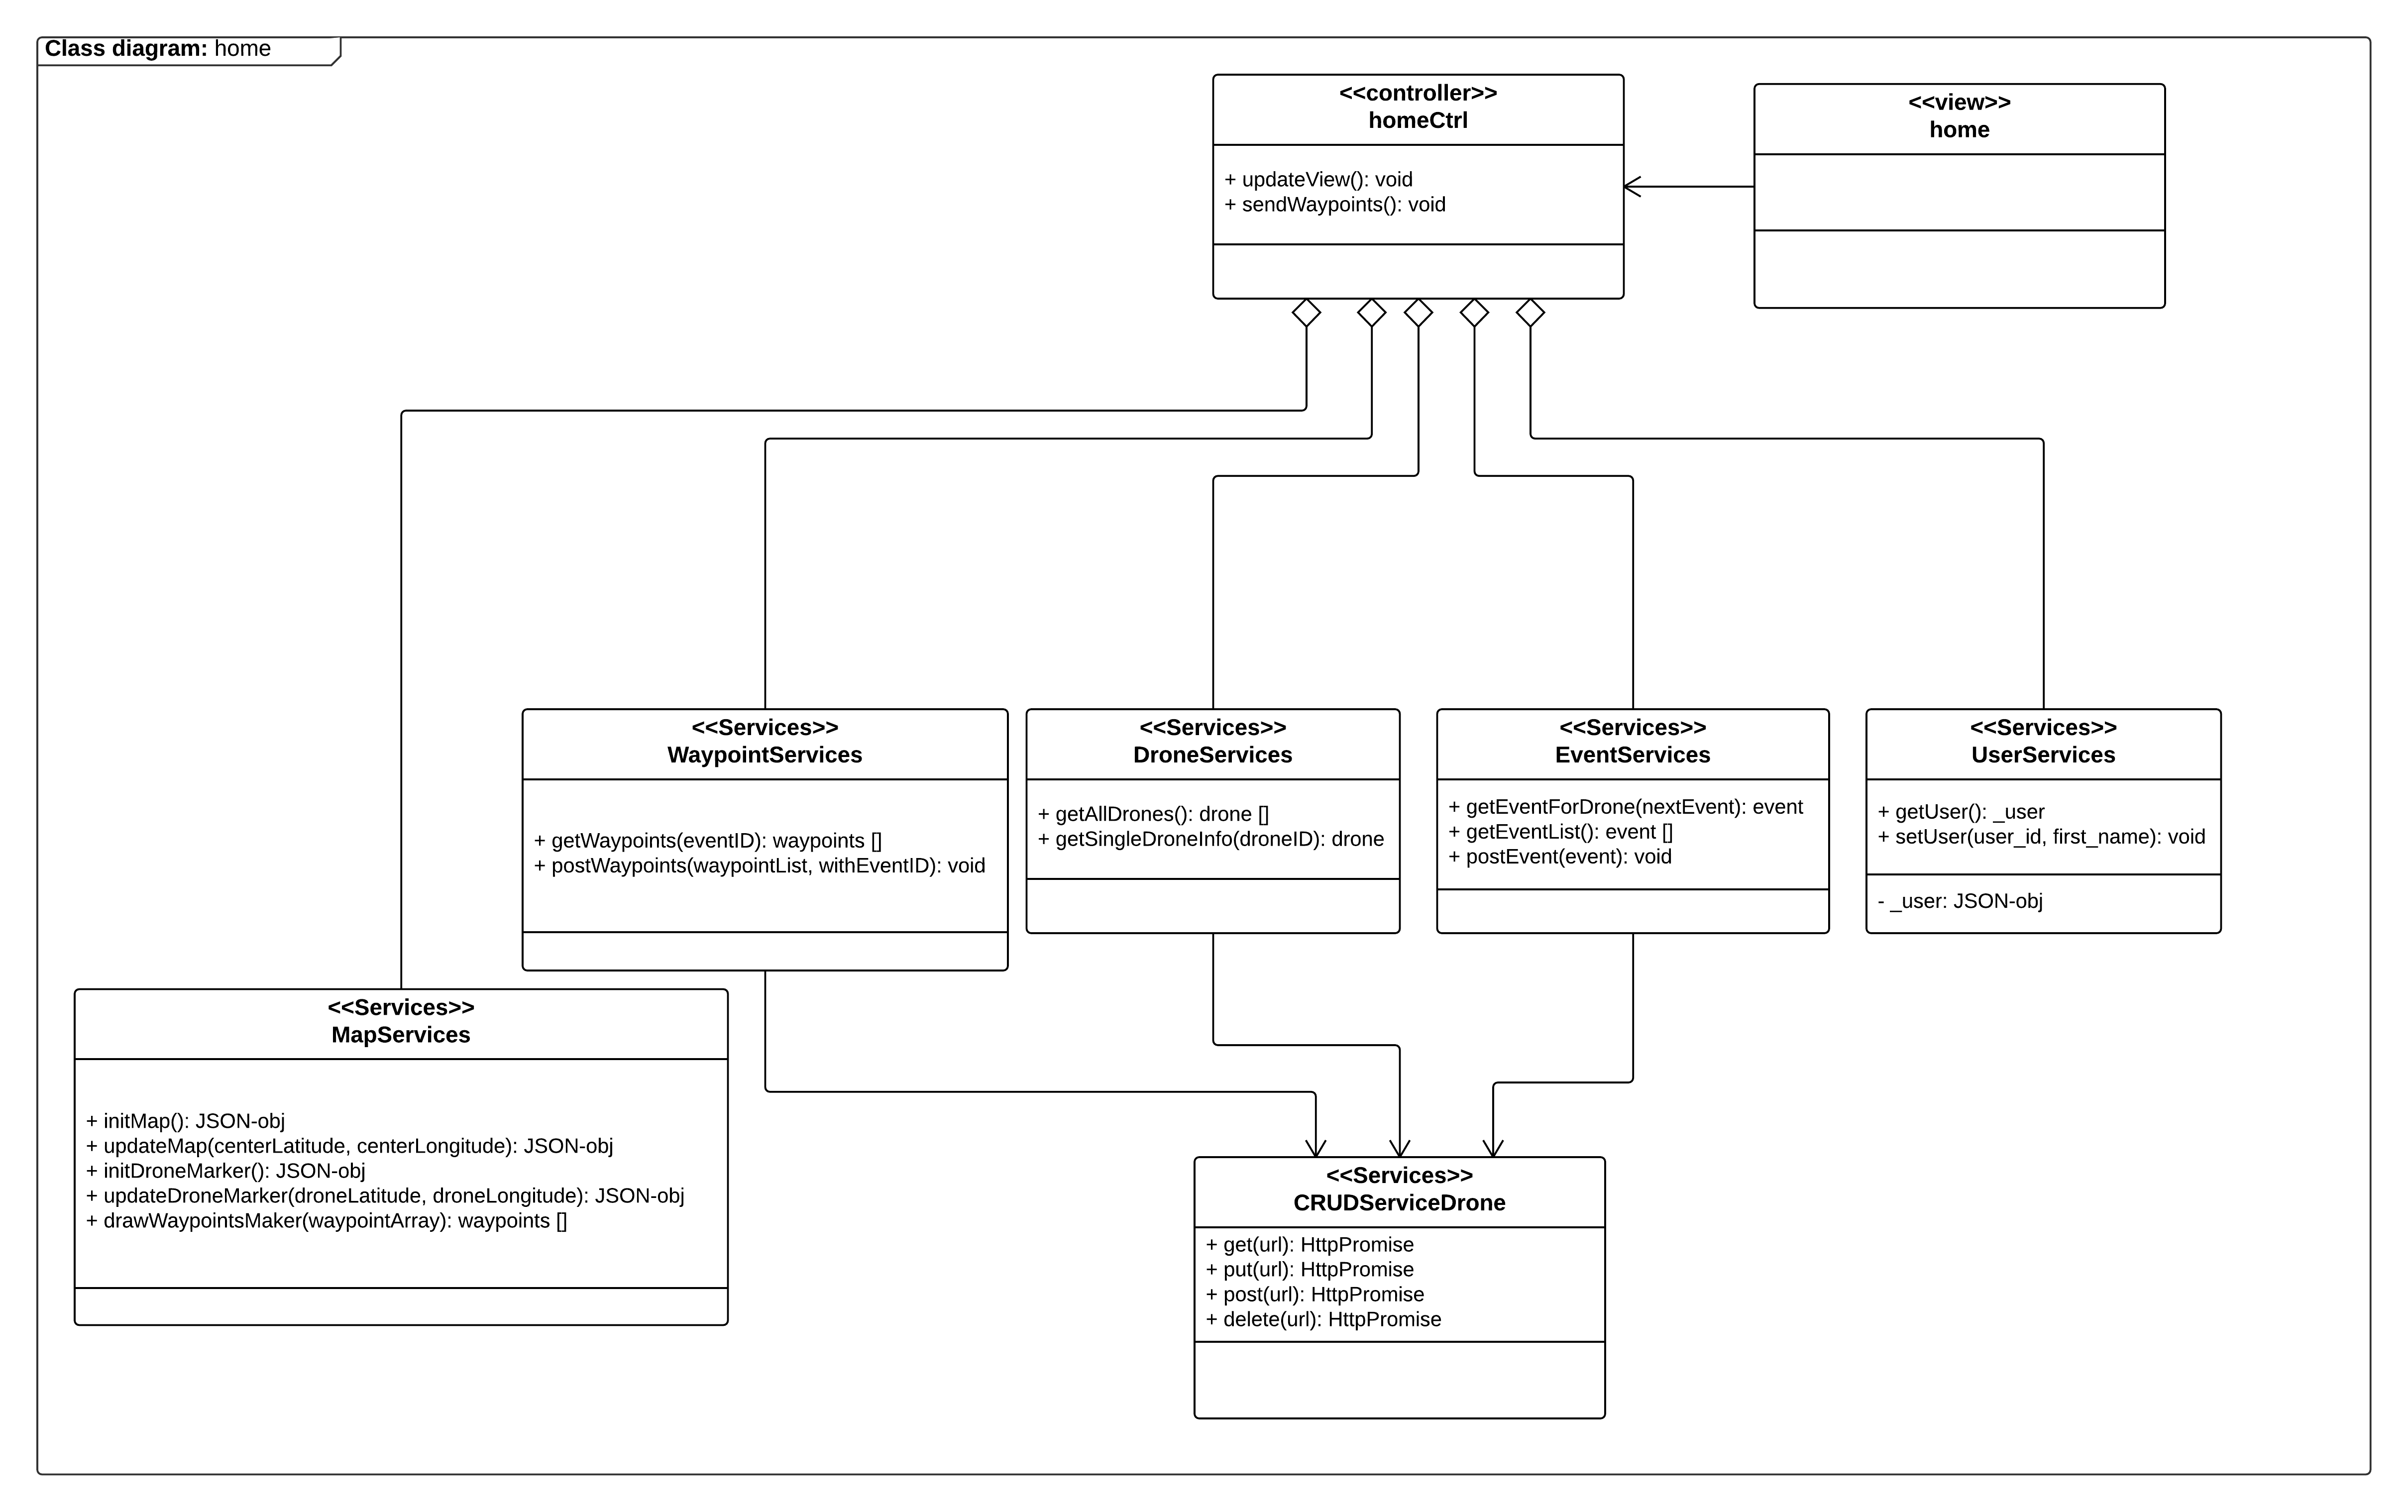
\includegraphics[width=1.1\textwidth]{Billeder/klasse_diagrammer/home_class_diagram.png}
	\vspace{-0.5cm}
	\caption{Klassediagram home}
	\label{fig:classDiagram_home}
\end{figure}
